\documentclass[12pt]{standalone}

\usepackage{xcolor}
\usepackage[prefix=solar-]{xcolor-solarized}

\usepackage{tikz}

\begin{document}
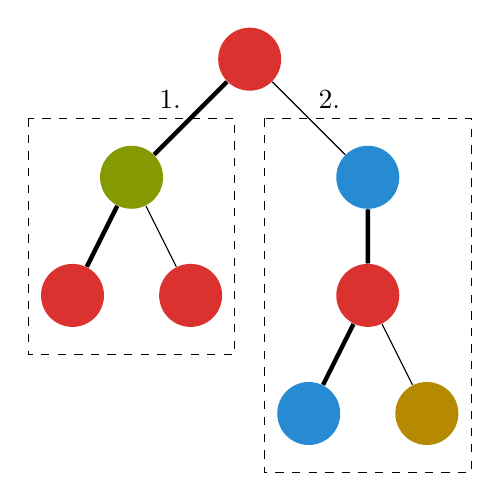
\begin{tikzpicture}[x=15mm,y=15mm]
    \begin{scope}[every node/.style={circle,fill,minimum size=8mm}]
        \node[solar-red] (A) at (0,1) {};

        \node[solar-green] (B) at (-1,0) {}
            child {node[solar-red] (D) {}}
            child {node[solar-red] (G) {}};

        \node[solar-blue] (I) at (1,0) {}
            child {node[solar-red] (J) {}
                child {node[solar-blue] (K) {}}
                child {node[solar-yellow] (L) {}}};
    \end{scope}

    \path
        (A) edge node[above left] {1.} (B) edge node[above right] {2.} (I);

    \path[ultra thick]
        (A) edge (B)
        (B) edge (D)
        (I) edge (J)
        (J) edge (K);

    \draw[dashed] (-1.875,0.5) rectangle (-0.125,-1.5);
    \draw[dashed] (0.125,0.5) rectangle (1.875,-2.5);
\end{tikzpicture}
\end{document}
